%
\chapter{Capturing gene expression in \platyfull{}'s brain}\label{ch:background}
%
\section{Platynereis dumerilii, an ideal organism of brain development studies}
     \subsection{General description}
     \platy{} is a marine annelid of the class Polychaeta, it has been established as one of the main marine animal models in the fields of evolutionary, developmental and neurobiological biology as well as ecology and toxicology \cite{hutchinson95,tessmar03,hardege99,dorresteijn90,fischer04,Fischer10}. As a member of the bilateria \platy{} has a defined bilateral symmetry.\\
     
     \platy populates shallow (no more than 3m) hard ocean floors around the world. It is commonly found in the Mediterranean sea, the north Atlantic coast of Europe as well as in the shallow seas surrounding Sri Lanka, Java and the Philippines. Eggs, embryos and larvae are roughly 160 $\mu$m while the adults can measure up to 6cm in length.
     
\begin{figure}[bth]
        \myfloatalign
        \subfloat[Larval form of \platy{}. Image: MPI for Developmental Biology.]
        {\label{fig:platynereis_larvae}
        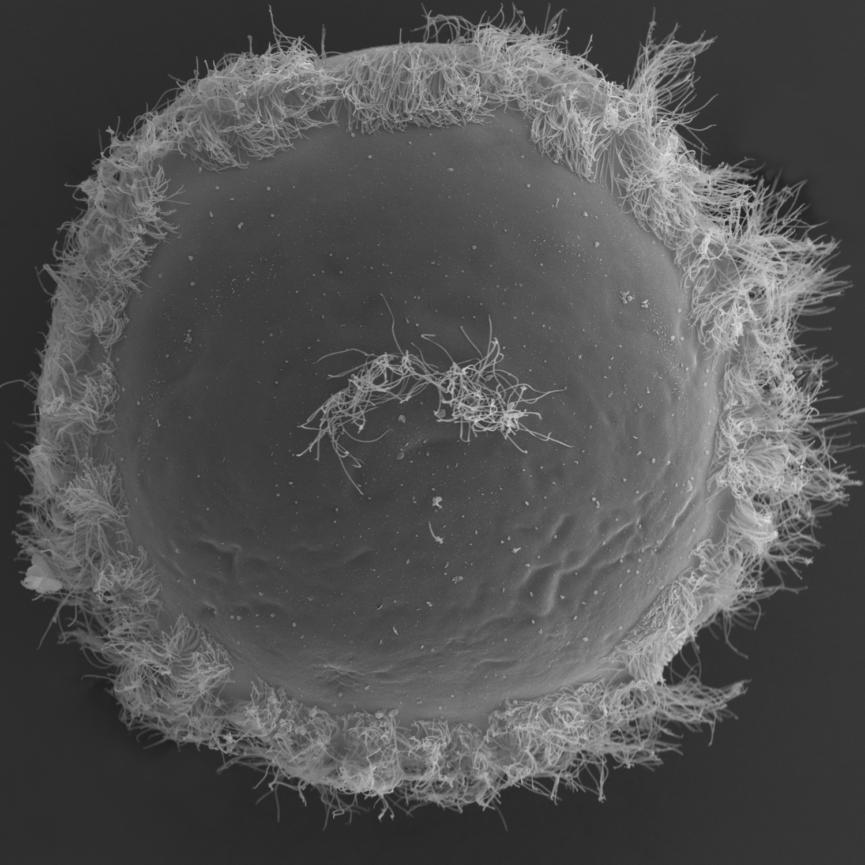
\includegraphics[width=.45\linewidth]{gfx/chapter1/platynereis_larva.jpg}} \quad
        \subfloat[Adult \platy{}. Image: Arendt group, EMBL]
        {\label{fig:platynereis_adult}%
         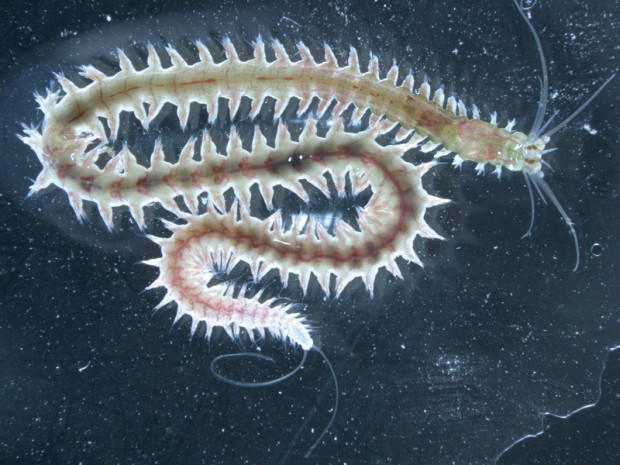
\includegraphics[width=.45\linewidth]{gfx/chapter1/platynereis_adult.jpg}}
        \caption{\platyfull{}'s larva and adult forms.}\label{fig:platynereis}
\end{figure}
     
     They are several reasons why \platy{} has been chosen as a model by numerous laboratories. In terms of evolution \platy{} shows several interesting characteristics. It belongs to the lophotrochozoan taxon of the bilaterian animals as opposed to most of the well established models animal which either belong to the ecdysozoans (\species{Caenorhabditis elegans}, \species{Drosophila melanogaster}) or the deuterostomes (mouse, human). Lophotrochozoans being extremely under represented, \platy{} as a model organism is essential to comparative approach on bilaterian biology.\\
     
     \platy{} also shows an exceptionally slow evolutionary lineage. It has even been described as a ``living fossil" for that reason \cite{Fischer10}. This means that the ancestral developmental characteristics of \platy{} are at an image of the common past of all bilaterians. To illustrate this fact an interesting example described in \cite{denes07,tessmar07} is the conserved molecular topography of the genes responsible for the development of the central nervous system between \platy{} and all vertebrates. This slow evolutionary rate confers \platy{} the advantage of being a link between fast evolving models like \species{drosophila} and vertebrates.\\
     
     In terms of practicality, \platy{} can easily be kept and bred in captivity producing offspring throughout the year \cite{fischer04}. The behavioural characteristics of \platy{} mating ritual have been well studied. The ``nuptial dance" happens on the water surface, male and female releasing the sperm and eggs synchronously, respectively. This activity is synchronized by pheromones released into the water \cite{zeeck98}. Over 2000 individuals can be produced within a single batch. Every new individual will undergo embryonic then larval development before reaching \platy{}'s adult form.\\

 
     \subsection{Larval development}
    Similarly to the other polychaetes, the larval development of \platy{} can be decomposed into three main anatomical stages: the trochophore, the metotrochophore and the nectochaete. The trochophore is spherical and moves via a equatorial belt of ciliated cells as well as an apical organ possessing a ciliary tuft \cite{rouse99,nielsen04} as seen on figure \ref{fig:platynereis_larvae} and schematically on figure \ref{fig:platynereis_larvae_scheme}. the metotrochophore stage is characterized by the development of a slightly elongated segmented trunk compared to that of the trochophore \cite{hacker98}. The next stage is the nectochaete larvae that resembles the adult (figure \ref{fig:platynereis_adult}) in most of the traits especially with parapodial appendages used for swimming and crawling \cite{hacker98}. This traditional subdivision has been applied to \platy{} \cite{hauenschild69}.\\
    
\begin{figure}[bth]
\begin{center}
  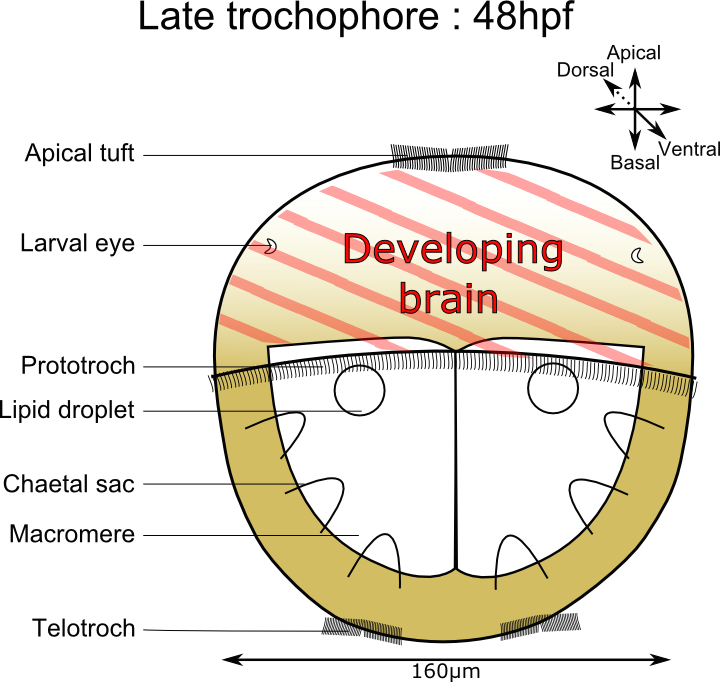
\includegraphics[width=0.6\linewidth]{gfx/chapter1/larvae48hpf.png}
\end{center}
  \caption{\platyfull{}'s larvea development at 48hpf or late trochophore. Striped in red is indicated the area which forms the developing brain of the larvae.}
  \label{fig:platynereis_larvae_scheme}
\end{figure}
    
    Aside from this purely anatomical subdivision, an additional staging systems exists and has become the norm for current studies. The development is measured in \textit{hours post fertilization} (hpf) at $18^{\circ}C$.
    
    A key factor making \platy{} such an interesting model to work with is the fact that after fertilization, the $\approx 2000$ larva will start developing at the exact same time, in a synchronous fashion. Furthermore, the larval development of \platy{} follows a very stereotypical pattern with very little variation from one individual to the other and even between batches provided the temperature is kept constant \cite{fischer04,dorresteijn90}. An example showing the similarity between individuals during development can be seen on figure \ref{fig:brain_comparison}. this is a very important feature as it allows biologists to repeat experiments on several individuals at a very close developmental stage even if they are from different batches.\\
    
\begin{figure}[bth]
  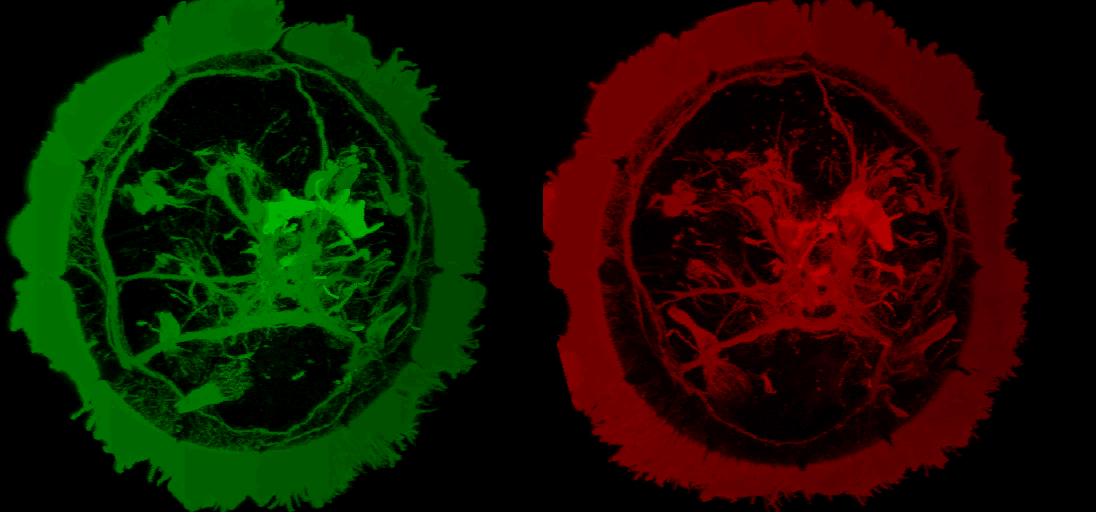
\includegraphics[width=\linewidth]{gfx/chapter1/brain_comparison.png}
  \caption{\platyfull{}'s stereotypical and synchronous development. In green and red are two different \platy{} individuals' with the same gene expression being highlighted. They show extremely similar patterns of development.}
  \label{fig:brain_comparison}
\end{figure}

	 Describing the entire development of \platy{} does not fall within the scope of this thesis. Indeed, we will only be interested in the brain of \platy{}'s larvae at 48hpf. Therefore, it is important to have an anatomical idea of what the brain looks like at this time in development and what inherent characteristics will be the most interesting to investigate.

\section{Gene expression in Platynereis' developing brain}
     \subsection{Platynereis' nervous development until 48hpf}
     The main purpose of this thesis is not to fully understand the patterns of development in \platy{}'s larval brain. Therefore we will only give a brief summary of what the main component of the brain are at 48hpf, the time point we will be interested in in the next chapters. \platy{}'s larval brain development is detailed in \cite{Fischer10}.\\
     From the early trochophore (24-26hpf) neural system development starts taking place. The apical ganglion forms at the apical tuft. It contains one sertonergic cell and a few neurons that link to the nerve of the ciliary band of the larva called the prototroch (see figure \ref{fig:platynereis_larvae_scheme} for better understanding). This allows the first movements of the larve thanks to the cialited cells of the prototroch.\\
     The mid-trochophore (26-40 hpf) sees the formation of the first cerebral commissure, it is a band of nerves interconnecting the ventral nerve cord and the brain. This trait is a typical feature of annelids brains. During this phase the apical ganglion becomes bigger with three more serotonergic cells.\\
     The late trochophore (40-48hpf)sees the formation of the second commissure in the ventral nerve cord. It is at the end of this stage that the brain starts to become more complexity with a notable increase in the number of neutrites.\\
     The data we will use in the rest of this thesis will not encapsulated the whole larvae, just the brain (see figure \ref{fig:platynereis_larvae_scheme}) thus excluding the ventral part of the nervous system. The best studied areas of the brain are the larval eyes, the developing adult eyes, the apical organ on the dorsal side. On the ventral side are located the mushroom bodies a pair of structures that are known to play a role in olfactory learning and memory in insects and annelids \cite{Tomer10}. A schematic representation of those areas is shown on figure \todo{FIGURE brain areas}.\\
     
     Even at a very early stage in a relatively simple organism, the brain quickly becomes a complex tissue. Cell types diverge and functional areas are formed. Before trying to understand more about \platy{}'s brain organization, it is interesting to ask the more general question about how complex tissues such as the brain are defined spatially.
     
          \subsection{Spatial organization of complex biological tissues like the brain}
     This section is not intended to demonstrate a specificity of the \platy{}'s brain, it is meant to ask some of the fundamental questions that intrinsically motivate the work presented in the rest of this thesis. Complex tissues, the obvious example of which is the brain, could be viewed as an interconnected mosaic of cells having different functions, working together to achieve the global function of the organ.\\
     
     If we look closely at this mosaic of cells, the spatial organisation of this mosaic is not random. Cells that serve the same function will often be close from each other, thus defining functional tissues. However, the spatial coherency of those tissues is not necessarily always the same. Some cell types could be formed of cells scattered inside another more spatially coherent tissue. To illustrate that fact, an interesting example is the difference between the spatial coherency of cells forming the neuronal tissue in the brain and cells forming a well defined region in the brain like the mushroom bodies. When asking the question, is it likely that this cell is fully surrounded by the same cell type, the extensions created by the axons of neurones will decrease this probability. Indeed, axons will grow through other types of tissues to reach their destination, making the overall spatial coherency of "neuronal" tissue smaller than very well spatially defined tissues.\\
     
     When trying to analyse the full structure of the brain with an automated method, keeping in mind that fact could prove important to improve the results. This fact and its consequences on the work presented in this method are further discussed in section \todo{cite section spatial clustering}.\\
     
     So far, we have only regarded organs and cell types as regarding their anatomical traits. But as mentioned in the introduction \ref{ch:introduction} the functional heterogeneity of complex tissues goes further that simple anatomical traits. We need to work on traits that fundamentally represent how cells are functioning.
     
     \subsection{Generalities about gene expression and development}  
     When speaking about developmental biology it it should be noted that the term ``cell" will be referring to eukaryotic cells and more specifically those of multicellular organisms. Every cell in a complex organism possesses the same genome, that is, the sum of all the genetic information contained in the cell (nucleus and other compartments). This fundamental homogeneity is in plain contradiction with the heterogeneity observed anatomically. If every cell has the exact same DNA, where does the great variability between cell types come from (what makes a neurone become a neurone and not a pancreatic cell). Answering this sort of questions defines the field of developmental biology.\\
     
     The short and rather complete answer to any developmental biology question actually is: same genome but different pattern of gene expression. As indeed gene expression is the central, most important, most studied cellular activity. Gene expression even is general common denominator of life as large parts of the mechanisms making up gene expression are actually shared by every living creature known to man.\\

     Of course to understand what gene expression is, we must first define what genes are. The precise definition of a gene is still controversial. The concept of a ``factor that conveys traits from parents to offspring" was laid by Gregor Mendel in 1866 \cite{mendel66} when the accepted theory at the time was based on blending inheritance where the traits of the parents appeared mixed in the offspring following a continuous gradient. The most recent published definition of a gene followed the publication of the ENCODE project \cite{feingold04}. It states that a gene is ``A gene is a union of genomic sequences encoding a coherent set of potentially overlapping functional products."\\

	Gene expression is the way cells express their genes. Expression of a gene is the process of transcribing the DNA of that particular gene. The product of gene expression is RNA molecules and there are several ways to look at gene expression. In a cell or tissue, at a given time point we can to choose to look whether a gene is expressed or not (binary expression) or how much a certain gene is expressed (quantitative expression).\\
	
	Most RNA molecules are translated into proteins that can have very different purposes some will directly serve in the cellular life as functional/structural agents (elements of the ATP synthase for example) others will have a regulatory effect on gene expression. In other terms the expression gene $a$, coding for protein $A$ might activate, accelerate, inactivate or decelerate expression of gene $b$ and potentially others. This outlines the complex interdependent regulatory system that is gene expression. For precise examples gene regulation see \cite{gossen92, shinozaki03,fuqua01,balmer02}.\\
	
	\todo{Add figure for gene expression Camille}
	
	During development mechanisms exist that allow gene expression to become differential as the divisions occur. This is how the asymmetrical axis (dorso-ventral, and basal-apical) of the body are defined. The main mechanism involves chemical gradients. The first of these gradient has to come from the original cell which musty contain some asymmetrically distributed chemical so that the first divisions lead to non identical cells. In the case of \platyfull{}, the body axis are defined  between 2hpf and 7hpf \cite{Fischer10}.\\
	
	As described, gene expression is the key factor during tissue development. The ability to study gene expression patterns has revolutionized the fields of developmental biology. Technological innovation has been the main driving factor of this revolution. In the next section we will present two methods to capture gene expression.


\section{Capturing gene expression in the laboratory}
     \subsection{In-situ hybridization assays}
     First proposed in 1969 by Pardue \cite{pardue69} and John \cite{joh69} independently, in-situ hybridization (ISH) used radioactive tritium labelled probes on a photographic emulsion to reveal on which chromosome particular genomic components were located. 
     In-situ hybridization is a technique that allows biologist to hybridize probes that are specific to some RNA or DNA sequence directly inside the tissues. When the probe finds a match and hybridizes it emits light thanks to a fluorescent label chemically attached. This allows biologist to map the expression of a gene in a thin slice of tissue.
     
\begin{figure}[h]
\centerline{\includegraphics[totalheight=0.4\textheight]{figures/data.png}}
\caption{Single cell in-situ hybridization expression data for 169 genes in the full brain of Platynereis. From the live tissue cut into 1 cell thick layers, every slice is stained with a reference gene and a gene of interest that will reveal the areas of expression under fluorescent microscopy. Every image is then divided into $\approx$ 1 cell large squares which allows the reconstruction of the 3D map of expression for one gene in the full brain. The process repeated 169 times for key genes in Platynereis development is the data generated by \cite{Tomer10}}\label{fig:insitu}
\end{figure}

    - FIG 2 : In situ hybridization principles
    - Explanations about the technique 

     \subsection{Building a referenced library of gene expression for Platynereis}
         - Stereotypical development allows one gene to be considered as reference
    - Different individuals are "replicates"
    - Mapping to a scaffold created by the reference gene

     \subsection{RNA sequencing}
    - FIG 3 : about RNA sequencing for tissues
    - Explanations about the technique
    - Obtaining the full transcriptome at once
    - Necessity of having the genome to map to or a list of known genes (primR) 
    - Discuss the starting RNA quantity 
    - Discuss the fact that gene expression is averaged over the tissue losing spatial information.

%
%
%
%
%




